\documentclass[11pt]{article}
%\documentclass[12pt]{article}
%\documentclass[12pt]{article}
%\documentclass[12pt,a4paper]{article}

\usepackage[percent]{overpic}
\usepackage{float}
\usepackage{pgfplots}
%\usepackage[cmbold]{mathtime}
%\usepackage{mt11p}
\usepackage{placeins}
\usepackage{amsmath}
\usepackage{amsthm}
\usepackage{color}
\usepackage{amssymb}
\usepackage{mathtools}
\usepackage{subfigure}
\usepackage{multirow}
\usepackage{epsfig}
\usepackage{listings}
\usepackage{enumitem}
\usepackage{rotating,tabularx}
%\usepackage[graphicx]{realboxes}
\usepackage{graphicx}
\usepackage{graphics}
\usepackage{epstopdf}
\usepackage{longtable}
\usepackage[pdftex]{hyperref}
%\usepackage{breakurl}
\usepackage{epigraph}
\usepackage{xspace}
\usepackage{amsfonts}
\usepackage{eurosym}
\usepackage{ulem}
\usepackage{footmisc}
\usepackage{comment}
\usepackage{setspace}
\usepackage{geometry}
\usepackage{caption}
\usepackage{pdflscape}
\usepackage{array}
\usepackage[round]{natbib}
\usepackage{booktabs}
\usepackage{dcolumn}
\usepackage{mathrsfs}
%\usepackage[justification=centering]{caption}
%\captionsetup[table]{format=plain,labelformat=simple,labelsep=period,singlelinecheck=true}%

%\bibliographystyle{unsrtnat}
\bibliographystyle{aea}
\usepackage{enumitem}
\usepackage{tikz}
\usetikzlibrary{decorations.pathreplacing}
%\def\checkmark{\tikz\fill[scale=0.4](0,.35) -- (.25,0) -- (1,.7) -- (.25,.15) -- cycle;}
%\usepackage{tikz}
%\usetikzlibrary{snakes}
%\usetikzlibrary{patterns}

%\draftSpacing{1.5}

\usepackage{xcolor}
\hypersetup{
colorlinks,
linkcolor={blue!50!black},
citecolor={blue!50!black},
urlcolor={blue!50!black}}

%\renewcommand{\familydefault}{\sfdefault}
%\usepackage{helvet}
%\setlength{\parindent}{0.4cm}
%\setlength{\parindent}{2em}
%\setlength{\parskip}{1em}

%\normalem

%\doublespacing
\onehalfspacing
%\singlespacing
%\linespread{1.5}

\newtheorem{theorem}{Theorem}
\newcommand{\bc}{\begin{center}}
\newcommand{\ec}{\end{center}}
\newtheorem{corollary}[theorem]{Corollary}
\newtheorem{proposition}{Proposition}
\newtheorem{definition}{Definition}
\newtheorem{axiom}{Axiom}
\newcommand{\ra}[1]{\renewcommand{\arraystretch}{#1}}

\newcommand{\E}{\mathrm{E}}
\newcommand{\Var}{\mathrm{Var}}
\newcommand{\Corr}{\mathrm{Corr}}
\newcommand{\Cov}{\mathrm{Cov}}

\newcolumntype{d}[1]{D{.}{.}{#1}} % "decimal" column type
\renewcommand{\ast}{{}^{\textstyle *}} % for raised "asterisks"

\newtheorem{hyp}{Hypothesis}
\newtheorem{subhyp}{Hypothesis}[hyp]
\renewcommand{\thesubhyp}{\thehyp\alph{subhyp}}

\newcommand{\red}[1]{{\color{red} #1}}
\newcommand{\blue}[1]{{\color{blue} #1}}

%\newcommand*{\qed}{\hfill\ensuremath{\blacksquare}}%

\newcolumntype{L}[1]{>{\raggedright\let\newline\\arraybackslash\hspace{0pt}}m{#1}}
\newcolumntype{C}[1]{>{\centering\let\newline\\arraybackslash\hspace{0pt}}m{#1}}
\newcolumntype{R}[1]{>{\raggedleft\let\newline\\arraybackslash\hspace{0pt}}m{#1}}

%\geometry{left=1.25in,right=1.25in,top=1.25in,bottom=1.25in}
\geometry{left=1in,right=1in,top=1in,bottom=1in}

\epstopdfsetup{outdir=./}

\newcommand{\elabel}[1]{\label{eq:#1}}
\newcommand{\eref}[1]{Eq.~(\ref{eq:#1})}
\newcommand{\ceref}[2]{(\ref{eq:#1}#2)}
\newcommand{\Eref}[1]{Equation~(\ref{eq:#1})}
\newcommand{\erefs}[2]{Eqs.~(\ref{eq:#1}--\ref{eq:#2})}

\newcommand{\Sref}[1]{Section~\ref{sec:#1}}
\newcommand{\sref}[1]{Sec.~\ref{sec:#1}}

\newcommand{\Pref}[1]{Proposition~\ref{prop:#1}}
\newcommand{\pref}[1]{Prop.~\ref{prop:#1}}
\newcommand{\preflong}[1]{proposition~\ref{prop:#1}}

\newcommand{\Aref}[1]{Axiom~\ref{ax:#1}}
\newcommand{\Dref}[1]{Definition~\ref{def:#1}}

\newcommand{\clabel}[1]{\label{coro:#1}}
\newcommand{\Cref}[1]{Corollary~\ref{coro:#1}}
\newcommand{\cref}[1]{Cor.~\ref{coro:#1}}
\newcommand{\creflong}[1]{corollary~\ref{coro:#1}}

\newcommand{\etal}{{\it et~al.}\xspace}
\newcommand{\ie}{{\it i.e.}\xspace}
\newcommand{\eg}{{\it e.g.}\xspace}
\newcommand{\etc}{{\it etc.}\xspace}
\newcommand{\cf}{{\it c.f.}\xspace}
\newcommand{\ave}[1]{\left\langle#1 \right\rangle}
\newcommand{\person}[1]{{\it \sc #1}}

\newcommand{\AAA}[1]{\red{{\it AA: #1 AA}}}
\newcommand{\YB}[1]{\blue{{\it YB: #1 YB}}}

\newcommand{\flabel}[1]{\label{fig:#1}}
\newcommand{\fref}[1]{Fig.~\ref{fig:#1}}
\newcommand{\Fref}[1]{Figure~\ref{fig:#1}}

\newcommand{\tlabel}[1]{\label{tab:#1}}
\newcommand{\tref}[1]{Tab.~\ref{tab:#1}}
\newcommand{\Tref}[1]{Table~\ref{tab:#1}}

\newcommand{\be}{\begin{equation}}
\newcommand{\ee}{\end{equation}}
\newcommand{\bea}{\begin{eqnarray}}
\newcommand{\eea}{\end{eqnarray}}
\newcommand{\bi}{\begin{itemize}}
\newcommand{\ei}{\end{itemize}}
\newcommand{\Dt}{\Delta t}
\newcommand{\Dx}{\Delta x}
\newcommand{\Epsilon}{\mathcal{E}}
\newcommand{\etau}{\tau^\text{eqm}}
\newcommand{\wtau}{\widetilde{\tau}}
\newcommand{\xN}{\ave{x}_N}
\newcommand{\Sdata}{S^{\text{data}}}
\newcommand{\Smodel}{S^{\text{model}}}
\newcommand{\del}{D}
\newcommand{\hor}{H}
\newcommand{\subhead}[1]{\mbox{}\newline\textbf{#1}\newline}
\setlength{\parindent}{0.0cm}
\setlength{\parskip}{0.4em}
\numberwithin{equation}{section}
\DeclareMathOperator\erf{erf}
%\let\endtitlepage\relax
\begin{document}
%\onehalfspacing
\begin{titlepage}
\title{Mobility, Mixing and Ergodicity: A Physically-Motivated Measure for Economic Mobility}
\author{Viktor Stojkoski \footnote{Macedonian Academy of Sciences and Arts,~\url{vstojkoski@manu.edu.mk}} \and Alexander Adamou\footnote{London Mathematical Laboratory,~\url{a.adamou@lml.org.uk}} \and Yonatan Berman\footnote{London Mathematical Laboratory,~\url{y.berman@lml.org.uk}} \and Colm Connaughton \footnote{London Mathematical Laboratory and University of Warwick,~\url{c.p.connaughton@warwick.ac.uk}} \and Ole Peters\footnote{London Mathematical Laboratory and Santa Fe Institute,~\url{o.peters@lml.org.uk}}\,\, \thanks{We thank...}}
%\date{First version: August 26, 2018\,\,\,\,\,\,\,\,\,\,\,\,\,\,\,\,\,\,\,\,\,\,\,\,Last revised: \today}
%\date{}
\date{\today}
\maketitle
%\bc
%\red{Preliminary version, please do not circulate}
%\ec
\begin{abstract}
\noindent 
\\
\\
\noindent\textbf{Keywords: mobility, inequality, ergodicity economics}
%\\
%\bigskip
\end{abstract}
\setcounter{page}{0}
\thispagestyle{empty}
%\nopagebreak
\end{titlepage}
\pagebreak \newpage
%\nopagebreak
\section{Introduction}\label{sec:introduction}
% What is mobility?
Economic mobility describes ``dynamic aspects of inequality''~\citep{Shorrocks1978}. It quantifies how wealth (or income\footnote{We focus on wealth in this paper, but it applies also to income}) ranks of individuals evolve over time. Intuitively, when mobility is high, ranks evolve quickly, and the chances of an individual to change her position in the wealth distribution over a given time period are high. When mobility is low, individuals are unlikely to change their rank in the distribution over time, or that it changes slowly.
% How is mobility typically measured?
\citet{Shorrocks1978} described several required properties of statistical measures of mobility and set the standard for such measures. Mobility measures are assumed to be derived from a transition matrix, a bistochastic matrix describing the conditional probabilities of individuals to move between different ranks over some time period. An example for such a measure, used extensively in the mobility literature, is the rank correlation, the correlation between individual wealth ranks in two points in time. Another canonical measure of mobility, used most typically in studies of intergenerational income mobility, is the intergenerational earnings elasticity (IGE), defined as the regression coefficient between log-incomes of parents and children.\footnote{In fact, the rank correlation and the IGE are both measures of immobility, and to consider them as measures of mobility one has to subtract them from 1.}
% Why are the typical measures problematic?
The standard statistical measures of mobility have several limitations. First, they are generally incomparable. For example, a rank correlation of 0.3 would have a different meaning if it corresponds to a period of one year or ten years. Second, for a given time period, it is not possible to tell whether some value of rank correlation is high or low, as this is a dimensionless quantity. Thus, rank correlation over some time period can only be high or low in comparison to other economies over a similar time period, or to other time periods of the same length.
In addition, the interpretation of the rank correlation depends on the underlying wealth distribution and its dynamics. The same rank correlation cannot be interpreted similarly when the underlying wealth distribution remains unchanged, and when it becomes more and more unequal.
The IGE has similar limitations, but also others. Most notably, the IGE is sensitive by-design to the level of inequality and not only to the transition matrix, as discussed in detail in the mobility literature (\eg~\citet{chettyETAL2014}).
% This paper
This paper introduces mixing time, a property of stochastic processes, as a measure of mobility. When wealth is an ergodic observable~\citep{PetersAdamou2018c}, and assuming the wealth distribution approaches a steady state, if the wealths of an arbitrary group of individuals is followed over time, the distribution of wealth within this group will gradually become similar to the steady-state wealth distribution. The characteristic time of this process is the mixing time. Put simply, it is the time scale over which individuals mix into the wealth distribution. When mixing is rapid, \ie the mixing time is short relative to the window of observation, we could interpret that as high wealth mobility. Slow mixing is interpreted as low mobility.
% We study RGBM
We then consider Reallocating Geometric Brownian Motion (RGBM~\citep{MarsiliMaslovZhang1998,LiuSerota2017,BermanPetersAdamou2019}) as a model for wealth dynamics and study mixing in this model. In RGBM, individual wealth undergoes random multiplicative growth, modeled as Geometric Brownian Motion (GBM), and is reallocated among individuals by a simple pooling and sharing mechanism. RGBM is a null model of an exponentially growing economy with social structure. It has three parameters representing economic growth, random shocks to individual wealth, and economic interaction among agents, quantified by the reallocation rate. This model is known to reproduce several important stylized facts. In particular, when the reallocation rate is positive, the wealth distribution converges to a stationary distribution with a Pareto tail. The model has both ergodic and non-ergodic regimes, characterized by the sign of the reallocation rate parameter~\citep{BermanPetersAdamou2019}.
% What is the mixing time in RGBM?
We find that in RGBM the mixing time scales with the inverse of the reallocation rate. As the reallocation rate becomes higher, \ie when a larger share of each individual's wealth is pooled and then shared per unit time, mixing time becomes shorter proportionally, and mobility increases. As the reallocation rate approaches zero, mixing times get longer, and mobility lower. Since decreasing reallocation rates also lead to increasing inequality, this result is in line with the empirical observation that as inequality increases mobility decreases, and vice versa~\citep{corak2013}.
% Mixing time and standard measures
\YB{Here we need to describe how mixing time and rank correlation or other standard measures are related in RGBM}
% Mixing in non-ergodic systems
In practice, many economic systems are best modeled as non-ergodic~\citep{Peters2019b}. In particular,~\citet{BermanPetersAdamou2019} argue that the US economy is best described in RGBM as one in which wealth is systematically reallocated from poorer to richer, \ie the reallocation rate is negative. In such a case there is no mixing, so the mixing time is infinite. Thus, measuring mobility using standard measures under this regime may be misleading. The thorough study of RGBM in this regime is outside of the scope of this paper and left for future work.
% Plan
The paper is organized as follows.~\Sref{mixingtime} discusses the concept of mixing time and how it provides a physically-motivated measure for mobility.~\Sref{rgbm} studies mobility using mixing times in reallocating geometric Brownian motion as a model for wealth. We conclude in~\Sref{conclusion}.

\section{Standard measures of economic mobility}\label{sec:mixingtime}

\subsection{Quantifying economic mobility}

%We measure the wealth $y_i(t)$ of a person $i$ in period $t$ in its rescaled transformation, $y_i(t) = x_i(t) / \langle x(t) \rangle_N$, where $x_i(t)$ is the actual wealth of the person and $N$ is the population size. The advantage of this transformation is that it leads to a dimensionless measurement unit for the wealth of a person, thus allowing for appropriate comparison of the wealth between different time periods.

Standard measures of economic mobility examine the properties of the bivariate joint distribution describing the wealth of the population in two different periods. Various methods have been developed for evaluating mobility under these circumstances, which, in general, exhibit similar characteristics. Therefore, in order to depict these characteristics we are going to utilize the three most widely used measures of economic mobility: the Spearman rank correlation, the intragenerational earnings elasticity and the wealth transition matrix. 

\paragraph{Spearman rank correlation:} The Spearman rank correlation between the wealths corresponding to two different time periods, $t_m$ and $t_n$ ($t_m < t_n$) is defined as
\begin{align*}
    r_{t_m,t_n} &= 1 - \frac{6\sum_i \big(rg(x_i(t_m)) - rg(x_i(t_n))\big)^2}{N(N^2-1)},
\end{align*}
where $rg(\mathrm{x})$ is the rank transformation of $\mathrm{x}$, $x_i(t)$ is the wealth of individual $i$ in period $t$ and $N$ is the population size. This measure is bounded between $-1$ and $1$, with lower values suggesting greater economic mobility.

\paragraph{Intragenerational earnings elasticity:} The second measure is the intragenerational earnings elasticity, quantified via the slope $b_{t_m,t_n}$ of the regression
\begin{align*}
    x_i(t_n) &= b_0 + b_{t_m,t_n} x_i(t_m) + u_i,
\end{align*}
where $b_0$ is the intercept and $u_i$ is the error term. This is a simple linear regression and therefore,
\begin{align}
    b_{t_m,t_n} &= \mathrm{corr}(x(t_n),x(t_m)) \frac{\mathrm{var(x(t_n))}}{\mathrm{var(x(t_m))}},
    \label{eq:iee-estimation}
\end{align}
where $\mathrm{corr}(\mathrm{x},\mathrm{y})$ is the correlation between the variables $\mathrm{x}$ and $\mathrm{y}$ and $\mathrm{var}(\mathrm{x})$ is the variance of $\mathrm{x}$. As with the rank correlation, lower intragenerational earnings elasticity also indicates greater mobility. However, this measure is unbounded and may take on any real values.

\paragraph{Wealth transition matrix:} The last measure, disaggregates wealth rankings and summarizes economic mobility in a
transition matrix $\mathbf{A}$ in which cell entries $A_{kl}$ show the probability that an individual in wealth quantile $k$ in period $t_m$ is found in wealth quantile $l$ in period $t_n$. In a perfectly mobile economy, the entries of the transition matrix are all equal to each other. In an immobile economy, on the other hand, the largest values are concentrated in the diagonal entries.

\subsection{Limitations}

To illustrate the limitations of the standard measures, in Fig~\ref{fig:standard-mobility-measures} we construct an artificial example where we examine the economic mobility in a population of 9 individuals during 3 time periods. In the left-most panel of the figure, we show the dynamics of the wealth rankings. Besides this, we also highlight the amount of wealth owned by a person with a colored circle, with darker colored and larger circle implying a wealthier person. 
\begin{figure*}[t!]
\includegraphics[width=\linewidth]{figs/fig_mobility_measures.pdf}
\caption{\textbf{Performance of mobility measures. \textcolor{red}{Add caption.}} \label{fig:standard-mobility-measures}}
\end{figure*}

In our artificial economy, between the three periods, only the four individuals with largest wealth are able to change their status. In particular, in the second period, $t_2$ the second wealthiest person becomes the one with the most wealth, while the wealthiest person in the first period $t_1$ fails to second position. In addition, the third and fourth wealthiest persons change position. In period $t_3$, the dynamics are reversed, thus ending up with the same wealth rankings as in $t_1$. The only difference is that in this period, the wealth inequality increased, \ie, the rich got richer and the poor got poorer. 

As a result, the rank correlation tells us that the mobility was the same between $t_1$ and $t_2$, and $t_1$ and $t_3$, but overall between $t_1$ and $t_3$ there was no mobility ($r_{t_1,t_3} = 1$). The intragenerational earnings elasticity gives us similar results. In fact, since inequality increased in the last period, it further suggests that the economy became less mobile. 

The same conclusions hold when looking at the transition matrices estimated by dividing the wealth rankings in tertiles. An astonishing observation of the last measure is that the transition matrices between $t_1$ and $t_2$ and $t_2$ and $t_3$ suggest that there is a $1/3$ chance for an person belonging in the second tertile to climb to the richer tertile and vice versa. However, we structured our economy in a way that allows movement only between the persons belonging on the edge of the tertile. Hence, the transition matrices fail to adequately represent the movement of the typical person in the tertile.

Obviously, standard measures of economic mobility represent aggregate values of the changes in the wealth rankings of the individuals which constitute the population between two time periods. Therefore, they i) rely on a relevant time period for which the wealth rankings are compared, and ii) do not quantify the mobility of the typical representative of the population.

\section{Mixing time}

\subsection{What is a mixing time?}\label{sec:what}

Mixing time is able to overcome the limitations of standard economic mobility measures by providing an estimate for the characteristic time scale over which individuals mix into the wealth distribution. Think of the economy as a cup of coffee and the typical person's wealth as the milk you pour in the coffee. Mixing time quantifies the time required for the milk to blend with the coffee. This enables the measure to be used for appropriate comparison between different time periods and economies.

As we will see in the following when we will study the RGBM model, there is a direct relation between mixing time and standard mobility measures, whenever mixing time is a finite quantity. However, the standard measures may still indicate that there is mobility even when mixing time does not exist. This is because,  mixing time depends on the existence of mobility between \textit{every} quantile in the wealth distribution, whereas for standard measures it is enough for to have transitions only between two quantiles for mobility to exist. In other words, mixing time not only describes the capabilities of poor individuals to rise and become leading social actors, but also evaluates the time required for a rich person to fall in the social ladder. Therefore, we believe that our measure embodies the true concept of mobility.

\subsection{Measuring mixing time}

In physical terms, mixing describes the property of a dynamical system of being strongly intertwined. That is, any set of particles moving according to the laws of the dynamical system and satisfying a small spread of uncertainty in their initial conditions, follow paths that enter into any region of the phase space, and in a relatively ``uniform'' way. After a sufficient period of time, the mixing time, the percentage of the particles found within a particular region, is proportional to the volume of that region. 

As defined, mixing is strongly related to the concept of ergodicity. However, the latter is a much broader concept: A dynamical system is said to be ergodic if time-averages are equal to ensemble averages. Put differently, ergodicity only implies that every trajectory spreads around the phase space. Hence, every dynamical system that is mixing is also ergodic, but the opposite is not necessarily true.

The ergodicity indicates that in a mixing economy there is always a stationary distribution to which some rescaled transformation of a person's wealth converges. This characteristic can be utilized to develop an estimation procedure for mixing time. Fig~\ref{fig:mixing-time} gives an example for how to estimate mixing time, whereas the formal procedure is as follows:
\begin{enumerate}
    \item[\textbf{1.}] \textbf{Select stationary distribution:} Set a target distribution to which the rescaled transformation of wealth converges (black line in the inset plots);
    \item[\textbf{2.}] \textbf{Select typical representatives:} Select a subsample of the population constituted of people close to the typical representative (red dashed line in the inset plots). For example, this can be the persons whose wealth is closest to either the mean/median/mode wealth, depending on the properties of the stationary distribution;
    \item[\textbf{3.}] \textbf{Track wealth dynamics:} Track the wealth dynamics of each person in the subsample for a sufficient amount of time. Snapshots for the wealth distribution at several time periods are given in the inset plots of Fig~\ref{fig:mixing-time}.
    \item[\textbf{3.}] \textbf{Quantify the differences between the subsample and the stationary wealth distributions:} At certain time periods quantify the differences between the subsample wealth distribution and the stationary distribution. This can be done by utilizing usual statistical distribution distance measures such as the Kullblack-Leibler divergence, the Hellinger distance or the Kolmogorov-Smirnov statistic. In Fig~\ref{fig:mixing-time}, we plot the the log of one such statistic as a function of time with a blue line. In a mixing economy the statistic will exhibit three states. First, there will be a transient state in which the differences between the subsample and stationary wealth distributions will be large and stable. Next, there will be a mixing time state during which the two distributions will slowly converge towards each other, and the statistic will slowly decrease. Finally, there will be a stable state with no significant differences between the stationary and subsample wealth distributions; 
    \item \textbf{Estimate mixing time:} Estimate the slope of the regression in which the dependent variable is the log of the statistic an the independent is time (black dash-doted line in the figure). Take the data only for the mixing time state. Mixing time is the additive inverse of the reciprocal value of the slope ($-1 / slope$).
\end{enumerate}

\begin{figure*}[t!]
\includegraphics[width=\linewidth]{figs/fig_mixing_time.pdf}
\caption{\textbf{Mixing time.} Note: y-axis should be log of statistic. \textcolor{red}{Add caption.} \label{fig:mixing-time}}
\end{figure*}


\section{Mixing in a simple model of an economy}\label{sec:rgbm}

\subsection{Reallocating geometric Brownian motion}
To motivate the application of mixing time in economic systems, we utilize the RGBM model. Under RGBM, the dynamics of the wealth of person $i$ is specified as
\begin{align}
    \mathrm{d} x_i &= x_i \left( \mu \mathrm{d}t + \sigma \mathrm{d}W_i \right) - \tau \left( x_i - \langle x \rangle_N \right) \mathrm{d}t,
\label{eq:rgbm}
\end{align}
with $\mu > 0$ being the drift term, $\sigma > 0$ the noise amplitude, and $\mathrm{d}W_i$ is an independent Wiener increment, $W_i(t) =\int_0^t \mathrm{d}W_i$. In the equation $\tau$ is a parameter that quantifies reallocation of wealth. It implies that every year, everyone in the economy contributes a proportion $\tau$ of their wealth to a central pool, and then the pool is shared evenly across the population ($\langle x \rangle_N$ is per-capita wealth). The parameter aggregates a multitude of effects: collective investment in infrastructure, education, social programs, taxation, rents paid, private profits made etc. 

The dynamical behavior of RGBM is strictly dependent on the relation between $\tau$ and $\sigma$, and can be both ergodic and non-ergodic. Since mixing time is predicated on ergodic dynamics, we are going to focus on the ergodic regime which occurs when $\tau > \frac{\sigma^2}{2}$. Then, the model exhibits mean-reversion as each $x_i$ reverts to the population average $\langle x \rangle_N$. The large population approximation $\langle x(t) \rangle_N = \exp \left[\mu t\right]$ is valid, and it can be used to write a mean field equation for the dynamics of the rescaled wealth $y_i = x_i / \langle x \rangle_N$ as
\begin{align}
    d y &=   y \sigma d W - \tau (y - 1) dt.
    \label{eq:rescaled-rgbm}
\end{align}
Notice that the mean field representation leads to decoupling of the dynamics of each individual $i$, and hence we can neglect the subscript $i$ in equation~(\ref{eq:rescaled-rgbm}). This is an especially convenient form of RGBM which allows for deriving powerful analytical results regarding the properties of the model. For instance, we can derive  the stationary distribution for the rescaled wealth, which reads
\begin{align}
    p(y) &= \frac{(\theta - 1)^{\theta}}{\Gamma(\theta)} \exp{\big(-\frac{\theta - 1}{y}\big)} y^{-(1+\theta)},
    \label{eq:stationary-distributin}
\end{align}
where $\theta = 1 + \frac{2 \tau}{\sigma^2}$ and $\Gamma(\cdot)$ is the Gamma function.
This distribution exhibits a power law tail and in probability theory is known as the Inverse gamma distribution. \textbf{additional note}

\subsection{Mixing time in RGBM}

In RGBM, mixing time can be analytically estimated from its correlation function,
\begin{align}
    \mathrm{corr(y(t), y(t+\delta))} &= \exp\left[ -\tau \delta \right].
    \label{eq:rgbm-correlation}
\end{align}
The correlation function measures the statistical relation between observations of rescaled wealth at two different time points $t$ and $t-\delta$. 

Let us define the time period $t^*$ as the transition at which the distribution of the subsample converges to the stationary distribution. Then, we can reformulate of the stationary distribution in terms of this period as,
\begin{align*}
    \mathrm{corr(y(t^*), y(t))} &= \exp\left[ -\tau (t^* -t)\right],
    %\label{eq:rgbm-correlation}
\end{align*}
for any time period $t$ that belongs to the mixing time state. Obviously, the magnitude of any statistical measure $S(t)$ will be proportional to the value of this correlation, and its log will be of the form
\begin{align}
    \log (S(t)) &=  - \tau (t^*-t),
\end{align}
which implies that the mixing time in RGBM is $1/\tau$. The interpretation behind this result is fairly intuitive -- in RGBM economic mobility is uniquely explained by the reallocation term. In an economy in which reallocation from the rich to the poor is larger, there will be also more mixing. 

Fig~\ref{fig:rgbm-mixing-time} compares our analytical expression with numerical simulations where mixing time was estimated through the procedure described in Section 3.2. In the estimation procedure we chose Kolmogorov-Smirnov statistic as a statistical distance measure.
\begin{figure*}[t!]
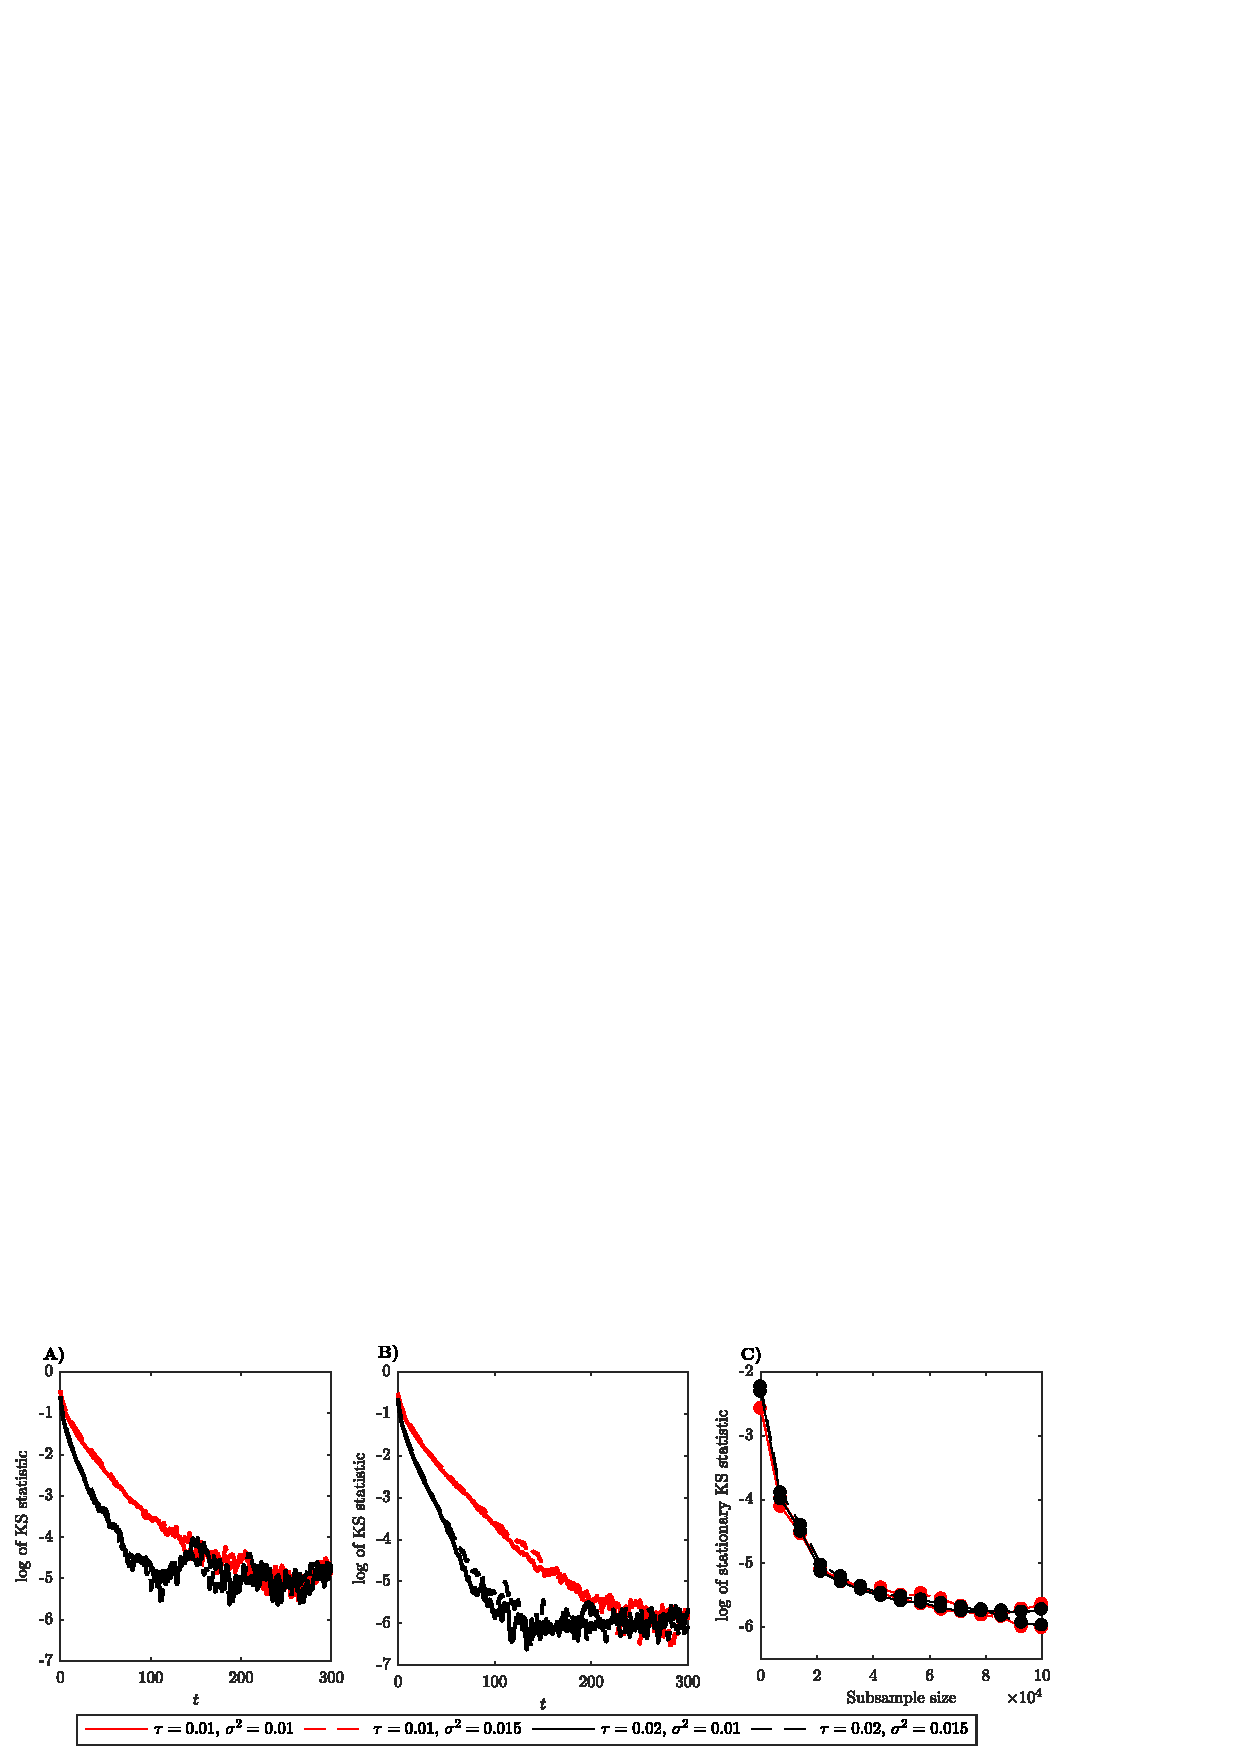
\includegraphics[width=10cm]{figs/fig_mixing_time_rgbm.png}
\caption{Mixing time in RGBM. \textcolor{red}{Describe the figure.}\label{fig:rgbm-mixing-time}}
\end{figure*}



\subsection{Mixing time and standard measures of mobility}\label{sec:measures}

Differently from the mixing time, in RGBM some of the standard measures mobility, besides being dependent on the reallocation parameter, are also determined by the noise amplitude $\sigma$. This is a consequence of \textbf{...}

\paragraph{Spearman rank correlation:} Simulations suggest that the log of the Spearman rank correlation is proportional to the additive inverse of the reallocation parameter $\tau$, but it is also related to the noise amplitude $\sigma$. This can be seen in  Fig.~\ref{fig:rgbm-spearman-correlation} where we plot the log of the rank correlation as a function of $\tau$ for various noise amplitudes.

\begin{figure*}[t!]
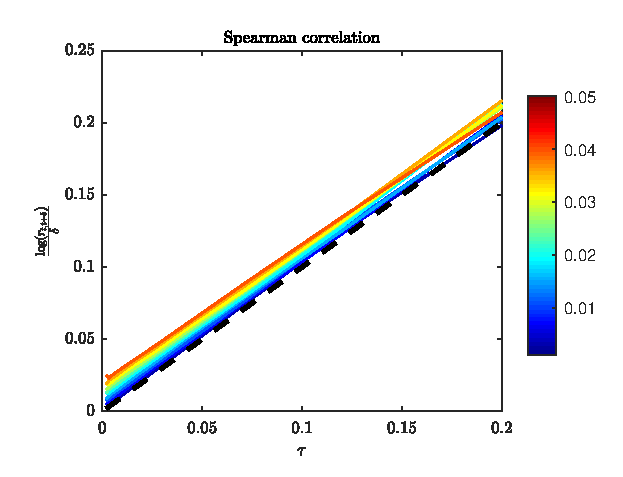
\includegraphics[width=10cm]{figs/fig_spearman_rgbm.eps}
\caption{\textbf{Spearman rank correlation in RGBM.} The colored lines correspond to numerical estimations of the stationary Spearman rank correlation in RGBM, color-mapped according to the magnitude of the noise amplitude. In the simulation, $\sigma^2 \in \left[ 0.001, 0.05\right]$, $\delta = 20$, $N = 10^4$.\label{fig:rgbm-spearman-correlation}}
\end{figure*}

\paragraph{Intragenerational earnings elasticity:} In RGBM, once the dynamics reaches a stationary state, the variance of $y(t)$ is invariant on time, \ie, the variances term in equation~(\ref{eq:iee-estimation}) cancel out. Hence, the  intergenerational earnings elasticity reduces simply to the correlation between observations corresponding to two different time periods as given by equation~(\ref{eq:rgbm-correlation}). This finding is confirmed in Fig.~\ref{fig:rgbm-iee}, where we show the log of the stationary intragenerational earnings elasticity as a function of the parameter $\tau$ and vary $\sigma^2$.

\begin{figure*}[t!]
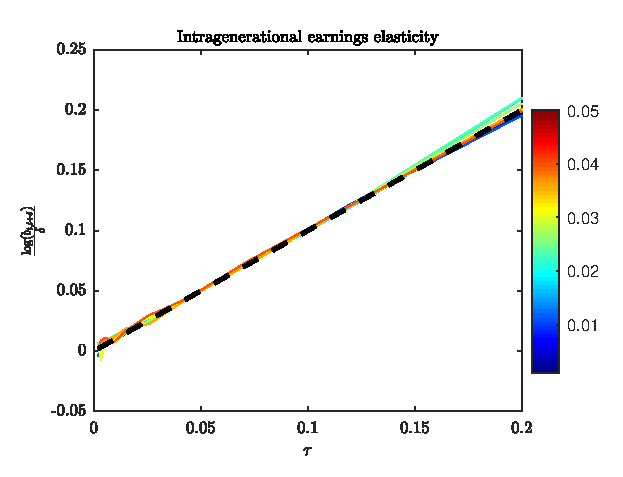
\includegraphics[width=10cm]{fig/fig_iee_rgbm.eps}
\caption{\textbf{Intragenerational earnings elasticity in RGBM.} The colored lines correspond to numerical estimations of the stationary Intragenerational earnings elasticity in RGBM, color-mapped according to the magnitude of the noise amplitude. In the simulation, $\sigma^2 \in \left[ 0.001, 0.05\right]$, $\delta = 20$, $N = 10^4$. \label{fig:rgbm-iee}}
\end{figure*}

\paragraph{Transition matrices:}

\textbf{Here introduce first hitting time and probably study it!}


\textbf{plot performance of standard measures, and mixing time}
\subsection{Mobility and inequality in reallocation geometric Brownian motion}\label{sec:inequality}

The ergodicity, and hence, stationarity allows us to use the stationary distribution in order analytically quantify standard welfare indices and subsequently use them to derive economic policies. For instance, the variance of the distribution can be used as a measure of economic inequality~\cite{berman2017empirical}. Its expression is
\begin{align}
\mathrm{var}(y) &= \frac{\sigma^2}{2 \tau - \sigma^2}.
\label{eq:rgbm-var}
\end{align}
Formally, economic inequality is defined as the extent of concentration in the distribution of wealth among the population. In this aspect, a higher variance implies that the total wealth in the economy is concentrated in few individuals, i.e., the society is more unequal.

In addition, the correlation function of the dynamics can be directly implemented as a measure of intragenerational social mobility, \textbf{describe connection between correlation function and measures of economic mobility}
\begin{align}
    \mathrm{corr(y(t), y(t+\delta))} &= \exp\left[ -\tau \delta \right],
    \label{eq:rgbm-mobility}
\end{align}
where $\delta$ quantifies the length of the period used for comparison of the wealth between individuals~\cite{liu2017correlation}.
Intragenerational social mobility measures the the feasibility of an individual to change their position in the wealth distribution. Since the system is ergodic, the correlation function can be used for deriving the mixing time, i.e., the time scale over which an individuals moves across the whole distribution. This is the relevant measure of immobility in the wealth dynamics of RGBM as it quantifies the amount of time needed for an individual to experience every wealth rank in the population. Its value is $1/\tau$, and a higher value indicates that it takes longer for an individual to visit all possible states of the distribution, thus making the economy less socially mobile.

Fig.~\ref{fig:rgbm-ineq-mobility} confirms the stationary dynamics of these two measures by plotting them as a function of time. The inset plot of the figure gives an example for the analytical power of the positive $\tau$ regime in RGBM. Namely, the figure visualizes the stationary Great Gatsby curve. This curve measures the relationship between inequality and social immobility, and has been used for developing social and financial policies. RGBM appropriately reproduces empirical observations by suggesting that economic inequality and social immobility are positively related~\cite{krueger2012rise}.

\begin{figure*}[t!]
\includegraphics[width=10cm]{fig0.eps}
\caption{Immobility and inequality in RGBM. \underline{\textbf{Scatter lines:}} Numerical estimation for the inequality and immobility, measured respectively via Eqs.~(\ref{eq:rgbm-var}) and~(\ref{eq:rgbm-mobility}), in a simulation or RGBM. The inset plot give the analytical relationship between inequality and mobility in RGBM, i.e. the Great Gatsby curve. \underline{\textbf{Parameters:}} We set $\mu = 0.021$, $\sigma^2 = 0.01$ and $N = 10^5$. The initial condition $x_i(0) = 1$ for all $i$.\label{fig:rgbm-ineq-mobility}}
\end{figure*}

\section{Conclusion}\label{sec:conclusion}
\bibliography{../LML_bibliography/bibliography}
%\clearpage
%\appendix
%\section{}\label{app:appA}
\end{document}